\subsection{Motywacja}
Partycjonowanie siatek jest bardzo ważnym podproblemem dla wielu dziedzin.
Ma między innymi zastosowanie dla sieci komputerowych, a także dla obliczeń równoległych, gdzie zależy nam,
aby problem podzielić na równe części pomiędzy węzły.
Jednym z takich problemów jest symulacja $2$D, dla której definiujemy zasady jej przebiegu oraz siatkę, na której ma się odbywać.
Przykładowo celem takiej symulacji może być zbadanie ruchu pieszego na mapie galerii handlowej, a następnie wyodrębnienie miejsc
zatłoczonych, które wymagają poprawek w projekcie.
Innym przykładem symulacji jest symulacja królików i kapusty przedstawiona na rysunku \ref{im:kroliki}.

Z racji na wielkość mapy taka symulacja często jest bardzo wymagająca obliczeniowo, dlatego dążymy do jej
zrównoleglenia.
Jedną z metod zrównoleglenia tego typu obliczeń jest podział siatki wejściowej pomiędzy węzły obliczeniowe,
tak by każdy węzeł zajmował się swoim obszarem.
Węzły mogą otrzymywać obszary równe pod względem wielkości pola, jeśli są to węzły homogeniczne, lub proporcjonalne do ich
możliwości obliczeniowych, jeśli są heterogeniczne.
Problemem, który towarzyszy zrównolegleniom jest narzut komunikacji.
Siatka pomimo podziału na części funkcjonuje jako całość, więc węzły muszą wiedzieć co dzieje się na granicach obszarów sąsiednich,
aby symulacja odbywała się prawidłowo.
W celu zminimalizowania narzutu komunikacyjnego należy więc zminimalizować długość granic pomiędzy obszarami.

\begin{figure}[h]
    \centering
    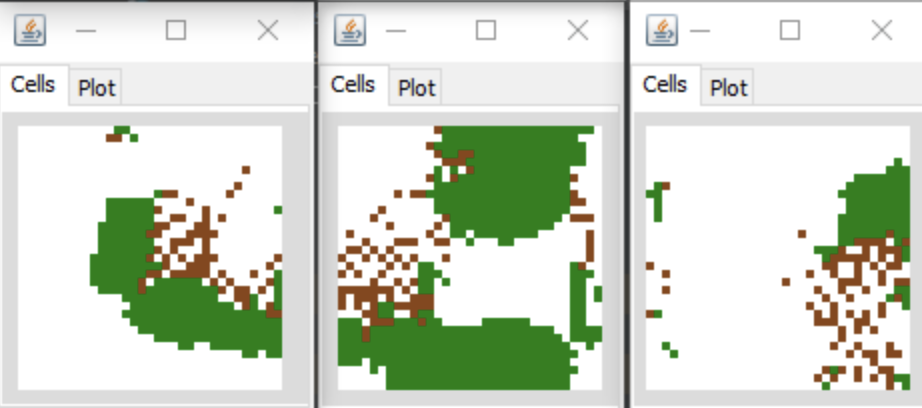
\includegraphics[width=0.6\linewidth]{images/kroliki}
    \caption{Fragment symulacji królików i kapusty. Króliki zjadają kapustę zwiększając swoją populację. Ze względu
    na zwiększoną populację królików i spadającą ilość pożywienia populacja królików spada, z czasem pozwalając
    populacji kapusty po raz kolejny się odrodzić. Każde okno obsługiwane jest przez osobny rdzeń procesora.}
    \label{im:kroliki}
\end{figure}

Patrząc na symulację jak ta przedstawiona na rysunku \ref{im:kroliki}, łatwo zaproponować bardzo dobry podział, ponieważ
siatka jest prostokątna.
Podział otrzymamy rysując pionowe oraz poziomie separatory na siatce.
Jeśli przyjmiemy właściwy sposób ich rysowania otrzymamy idealny podział zarówno pod względem wielkości pól, jak i
długości granic pomiędzy obszarami.
Problem przestaje być trywialny, jeśli siatka nie jest prostokątem lub chcemy, aby wyodrębnione obszary
siatki nie zostały podzielone między partycje, to znaczy należały zawsze do jednej partycji.
Często również z różnych powodów obliczenia nigdy nie odbędą się na pewnych obszarach siatki.
Mogą to być na przykład ściany na mapie galerii handlowej lub pomieszczenia, do których nie wchodzą klienci.
Chcemy aby tego typu obszary zostały w taki sposób ujęte w podziale siatki, aby uniknąć sytuacji, kiedy
jeden węzeł otrzyma do symulowania część siatki z obszarem, na którym symulacja nie będzie się odbywać.
Nie będzie on wtedy wykorzystywany do symulacji.
